

\tikzset{every picture/.style={line width=0.75pt}} %set default line width to 0.75pt        

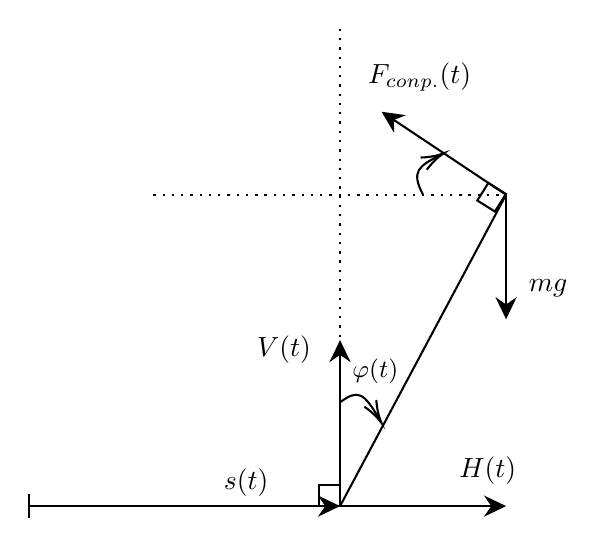
\begin{tikzpicture}[x=0.75pt,y=0.75pt,yscale=-1,xscale=1]
%uncomment if require: \path (0,300); %set diagram left start at 0, and has height of 300

%Straight Lines [id:da9082960361623723] 
\draw    (40,250) -- (187,250) ;
\draw [shift={(190,250)}, rotate = 180] [fill={rgb, 255:red, 0; green, 0; blue, 0 }  ][line width=0.08]  [draw opacity=0] (10.72,-5.15) -- (0,0) -- (10.72,5.15) -- (7.12,0) -- cycle    ;
\draw [shift={(40,250)}, rotate = 180] [color={rgb, 255:red, 0; green, 0; blue, 0 }  ][line width=0.75]    (0,5.59) -- (0,-5.59)   ;
%Straight Lines [id:da619700854654778] 
\draw    (270,100) -- (190,250) ;
%Straight Lines [id:da2680213245501296] 
\draw    (270,100) -- (270,157) ;
\draw [shift={(270,160)}, rotate = 270] [fill={rgb, 255:red, 0; green, 0; blue, 0 }  ][line width=0.08]  [draw opacity=0] (10.72,-5.15) -- (0,0) -- (10.72,5.15) -- (7.12,0) -- cycle    ;
%Straight Lines [id:da8310917143221241] 
\draw    (270,100) -- (212.5,61.66) ;
\draw [shift={(210,60)}, rotate = 393.69] [fill={rgb, 255:red, 0; green, 0; blue, 0 }  ][line width=0.08]  [draw opacity=0] (10.72,-5.15) -- (0,0) -- (10.72,5.15) -- (7.12,0) -- cycle    ;
%Straight Lines [id:da8347318970212223] 
\draw    (190,250) -- (267,250) ;
\draw [shift={(270,250)}, rotate = 180] [fill={rgb, 255:red, 0; green, 0; blue, 0 }  ][line width=0.08]  [draw opacity=0] (10.72,-5.15) -- (0,0) -- (10.72,5.15) -- (7.12,0) -- cycle    ;
%Straight Lines [id:da0962341838743137] 
\draw    (190,250) -- (190,173) ;
\draw [shift={(190,170)}, rotate = 450] [fill={rgb, 255:red, 0; green, 0; blue, 0 }  ][line width=0.08]  [draw opacity=0] (10.72,-5.15) -- (0,0) -- (10.72,5.15) -- (7.12,0) -- cycle    ;
%Straight Lines [id:da41784265135185517] 
\draw  [dash pattern={on 0.84pt off 2.51pt}]  (190,20) -- (190,250) ;
%Curve Lines [id:da2623450692945557] 
\draw    (190,200) .. controls (198.64,193.6) and (201.44,195.19) .. (209.03,208.3) ;
\draw [shift={(210,210)}, rotate = 240.4] [color={rgb, 255:red, 0; green, 0; blue, 0 }  ][line width=0.75]    (10.93,-3.29) .. controls (6.95,-1.4) and (3.31,-0.3) .. (0,0) .. controls (3.31,0.3) and (6.95,1.4) .. (10.93,3.29)   ;
%Straight Lines [id:da07376152116457713] 
\draw  [dash pattern={on 0.84pt off 2.51pt}]  (100,100) -- (270,100) ;
%Curve Lines [id:da8812105788162867] 
\draw    (230,100) .. controls (223.98,88.6) and (227.89,86.23) .. (238.3,80.87) ;
\draw [shift={(240,80)}, rotate = 512.78] [color={rgb, 255:red, 0; green, 0; blue, 0 }  ][line width=0.75]    (10.93,-3.29) .. controls (6.95,-1.4) and (3.31,-0.3) .. (0,0) .. controls (3.31,0.3) and (6.95,1.4) .. (10.93,3.29)   ;
%Shape: Rectangle [id:dp47533838253981786] 
\draw   (180,240) -- (190,240) -- (190,250) -- (180,250) -- cycle ;
%Shape: Rectangle [id:dp26114282721727233] 
\draw   (256.14,102.77) -- (261.45,94.3) -- (269.92,99.61) -- (264.61,108.08) -- cycle ;

% Text Node
\draw (148.75,238.63) node   [align=left] {\begin{minipage}[lt]{22.1pt}\setlength\topsep{0pt}
$\displaystyle s(t)$
\end{minipage}};
% Text Node
\draw (246,224.5) node [anchor=north west][inner sep=0.75pt]   [align=left] {$\displaystyle H(t)$};
% Text Node
\draw (148.5,166.5) node [anchor=north west][inner sep=0.75pt]   [align=left] {$\displaystyle V(t)$};
% Text Node
\draw (202,35) node [anchor=north west][inner sep=0.75pt]   [align=left] {$\displaystyle F_{conp.}(t)$};
% Text Node
\draw (279.5,139.5) node [anchor=north west][inner sep=0.75pt]   [align=left] {$\displaystyle mg$};
% Text Node
\draw (194.5,177.5) node [anchor=north west][inner sep=0.75pt]  [font=\small] [align=left] {$\displaystyle \varphi ( t)$};


\end{tikzpicture}